\documentclass{standalone}
\usepackage{tikz}
\usepackage{amsmath}
\usepackage[T1]{fontenc}
\tikzset{
    process/.style={draw, rectangle, rounded corners, fill=yellow!20, minimum width=1cm, auto, on grid, minimum height=1cm, align=center},
    process4/.style={draw, font=\fontsize{8}{9.6}\selectfont, rectangle, rounded corners, fill=yellow!20, text width=3cm, auto, on grid, align=center},
    decision/.style={draw, font=\fontsize{8}{9.6}\selectfont, rectangle, rounded corners, fill=red!20, text width=3cm, minimum height=1cm, auto, on grid, align=center},
    process2/.style={draw, font=\fontsize{10}{12}\selectfont, rectangle, rounded corners, fill=cyan!20, text width=4cm, auto, on grid, align=center},
    process3/.style={draw, font=\fontsize{10}{12}\selectfont, rectangle, rounded corners, fill=cyan!20, rotate=-90, auto, on grid, align=center},
    vecArrow/.style={thick, decoration={markings,mark=at position 1 with {\arrow[semithick]{open triangle 60}}},
        double distance=1.4pt, shorten >= 5.5pt,
        preaction = {decorate},
        postaction = {draw,line width=1.4pt, white,shorten >= 4.5pt}},
    vecArrow1/.style={thick, decoration={markings,mark=at position 0.9 with {}},
        double distance=1.4pt, shorten >= 5.5pt,
        preaction = {decorate},
        postaction = {draw,line width=1.4pt, white,shorten >= 4.5pt}},
    innerWhite/.style={semithick, white,line width=1.4pt, shorten >= 4.5pt},
}

\usetikzlibrary{arrows, decorations.markings, arrows.meta,positioning,shadows,shapes.geometric,automata,positioning,fit,arrows.meta,calc,bending}

% Define your tikz styles here
\tikzstyle{process}=[draw,rectangle, rounded corners, fill=yellow!20, minimum width=1cm, auto, on grid, minimum height=1cm, align=center]
\tikzstyle{process4}=[draw,font=\fontsize{8}{4.8}, rectangle, rounded corners,fill=yellow!20, text width=3cm, auto,on grid,align=center]
\tikzstyle{decision}=[draw,font=\fontsize{8}{4.8}, rectangle, rounded corners,fill=red!20, text width=3cm, minimum height=1cm, auto,on grid,align=center]
\tikzstyle{process2}=[draw,font=\fontsize{10}{4.8}, rectangle, rounded corners,fill=cyan!20, text width=4cm, auto,on grid,align=center]
\tikzstyle{process3}=[draw, font=\fontsize{10}{4.8}\selectfont,rectangle, rounded corners,fill=cyan!20, rotate=-90, auto,on grid,align=center]

\tikzstyle{vecArrow} = [thick, decoration={markings,mark=at position
   1 with {\arrow[semithick]{open triangle 60}}},
   double distance=1.4pt, shorten >= 5.5pt,
   preaction = {decorate},
   postaction = {draw,line width=1.4pt, white,shorten >= 4.5pt}]
\tikzstyle{vecArrow1} = [thick, decoration={markings,mark=at position
   0.9 with {}},
   double distance=1.4pt, shorten >= 5.5pt,
   preaction = {decorate},
   postaction = {draw,line width=1.4pt, white,shorten >= 4.5pt}]
\tikzstyle{innerWhite} = [semithick, white,line width=1.4pt, shorten >= 4.5pt]

\usepackage{graphicx} % for including images

\usepackage{overpic} % for overlaying text on images

\begin{document}
\resizebox{0.8\textwidth}{!}{\begin{tikzpicture}
\tikzstyle{process}=[draw,rectangle, rounded corners, fill=yellow!20, minimum width=1cm, auto, on grid, minimum height=1cm, align=center]
\tikzstyle{process4}=[draw,font=\fontsize{8}{4.8}, rectangle, rounded corners,fill=yellow!20, text width=3cm, auto,on grid,align=center]
\tikzstyle{decision}=[draw,font=\fontsize{8}{4.8}, rectangle, rounded corners,fill=red!20, text width=3cm, minimum height=1cm, auto,on grid,align=center]
\tikzstyle{process2}=[draw,font=\fontsize{10}{4.8}, rectangle, rounded corners,fill=cyan!20, text width=4cm, auto,on grid,align=center]
\tikzstyle{process3}=[draw, font=\fontsize{10}{4.8}\selectfont,rectangle, rounded corners,fill=cyan!20, rotate=-90, auto,on grid,align=center]

\tikzstyle{vecArrow} = [thick, decoration={markings,mark=at position
   1 with {\arrow[semithick]{open triangle 60}}},
   double distance=1.4pt, shorten >= 5.5pt,
   preaction = {decorate},
   postaction = {draw,line width=1.4pt, white,shorten >= 4.5pt}]
\tikzstyle{vecArrow1} = [thick, decoration={markings,mark=at position
   0.9 with {}},
   double distance=1.4pt, shorten >= 5.5pt,
   preaction = {decorate},
   postaction = {draw,line width=1.4pt, white,shorten >= 4.5pt}]
\tikzstyle{innerWhite} = [semithick, white,line width=1.4pt, shorten >= 4.5pt]
\node[inner sep=0pt] (tri) at (4,-0.35){{\scalebox{.12}{   
\begin{overpic}[scale=5]{figures/triangulation}
\put(-2,15){$C_L$}
\put(15,12){$X_L$}
\put(0,5){$Y_L$}
\put(92,14){$C_R$}
\put(91,5){$Y_R$}
\put(102,18){$X_R$}
\put(44,-3){R}
\put(44,13.5){T}
\put(30,9.5){{\fontsize{86}{36}\selectfont triangulation}}
\put(24,47){$Z_L$}
\put(6,47){$u_L$}
\put(-3,39){$v_L$}
\put(50,59){$P_0$}
\put(63,59){$P_1$}
\put(74,47){$Z_R$}
\put(70,42){$u_R$}
\put(62,33){$v_R$}
\end{overpic}}}};
\node[inner sep=0pt] (1) at (-4,0.8){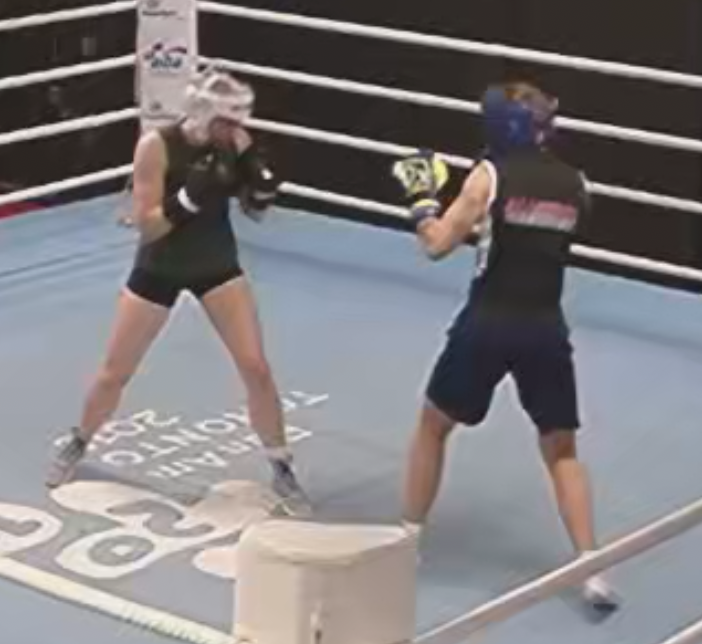
\includegraphics[width=.1\textwidth]{figures/p1.png}};
\node at (-4,-0.35) {\vdots};
\node[inner sep=0pt] (2) at (-4,-1.5) {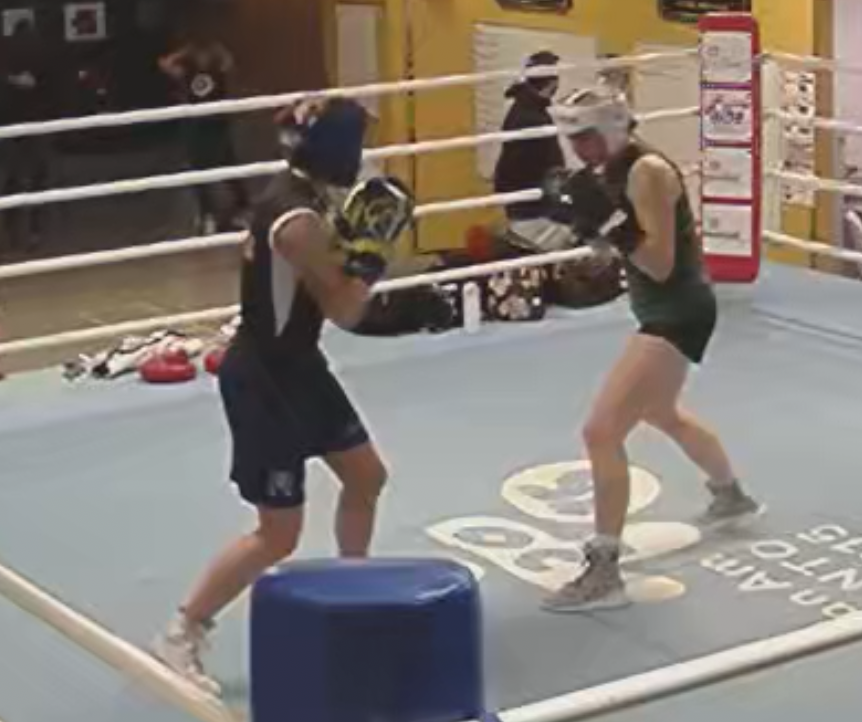
\includegraphics[width=.1\textwidth]{figures/p2.png}};

\node[process3] (yolo) at (-2.2,-0.4) {Yolov8};
\draw[vecArrow] (-3.1,-0.4) tonode[anchor=west, rotate=-90] {{$\mathrm{view}_j$}} (yolo);
\node[process3] (xmem) at (-1,-0.4) {XMem};
\node[process3] (vitpose) at (1,-0.4) {ViT Pose};
\draw[vecArrow] (yolo) tonode[anchor=west, rotate=-90] {$\mathbf{bboxes}$} (xmem) ;
\node[process3] (epipolar) at (0,-0.4){epipolar constraints};
\draw[vecArrow] (xmem) tonode[anchor=west, rotate=-90] {$\mathbf{ids}$} (epipolar);

% \node[process4] (diffusion filter) at (6.9,-0.35){diffusion filter};
% \draw[vecArrow] (sort1) |-  (epipolar);
\draw[vecArrow] (epipolar) tonode[anchor=west, rotate=-90] {$\mathrm{id}$} (vitpose);

\draw[vecArrow] (vitpose) tonode[anchor=west, rotate=-90] {$\mathbf{J}_{2D}$} (tri);

\node[process] (kinematics) at (8.5,-0.35) {Kinematics\\Optimization};
\node[process2] (prior) at (8.5,0.75) {GMM Prior, Vposer};
\node[process2] (loss) at (8.5,-1.5) {$\mathrm{L}_\text{2D}$, $\mathrm{L}_\text{3D}$, $\mathrm{L}_\text{reg}$, $\mathrm{L}_\text{smooth}$};
\draw[vecArrow] (loss) to (kinematics);
\draw[vecArrow] (prior) to (kinematics);
\draw[vecArrow] (tri) -- node[above] {$\mathbf{J}_{2D}$} node[below] {$\mathbf{J}_{3D}$} (kinematics);
% \draw[vecArrow] (diffusion filter) to (kinematics);

\node[inner sep=0pt] (smpl2) at (11,-0.35) {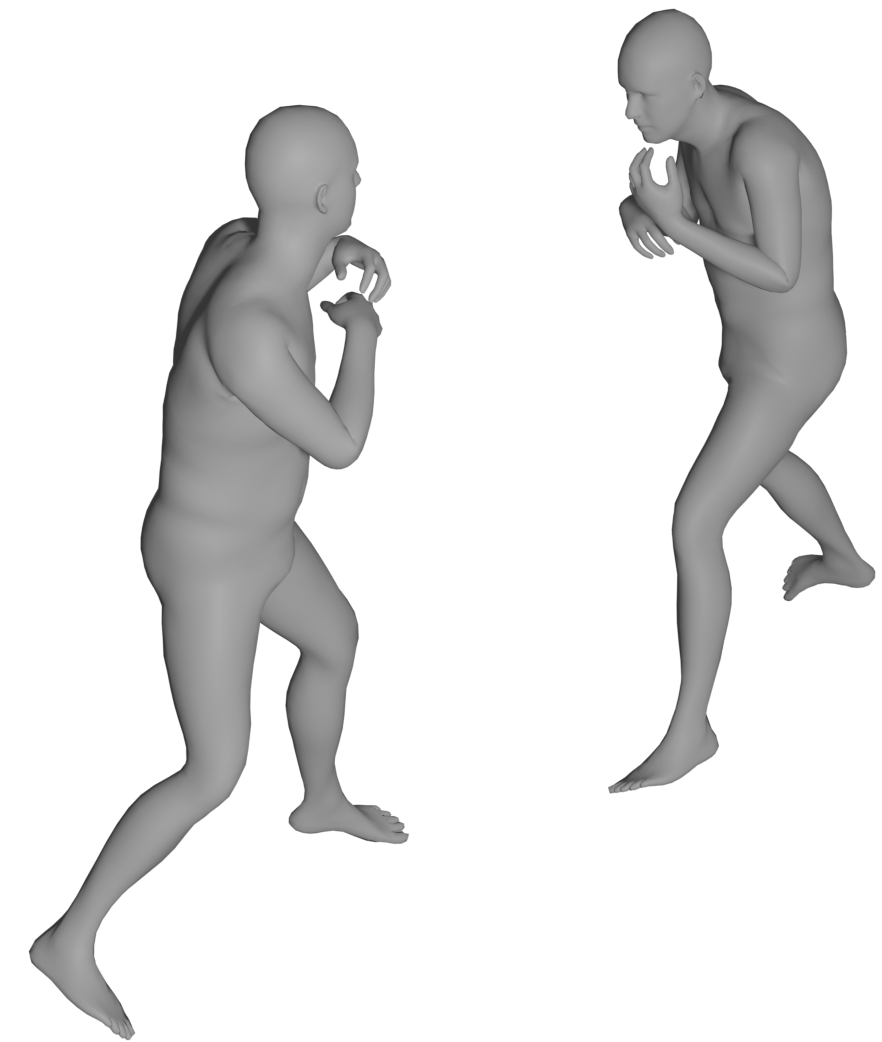
\includegraphics[width=.1\textwidth]{figures/smpl2.png}};
\draw[vecArrow] (kinematics) tonode[anchor=south] {\scriptsize{$\mathbf{\theta}$, $\mathbf{\beta}$}} (smpl2);
\node[inner sep=0pt] (smpl) at (-4,-4){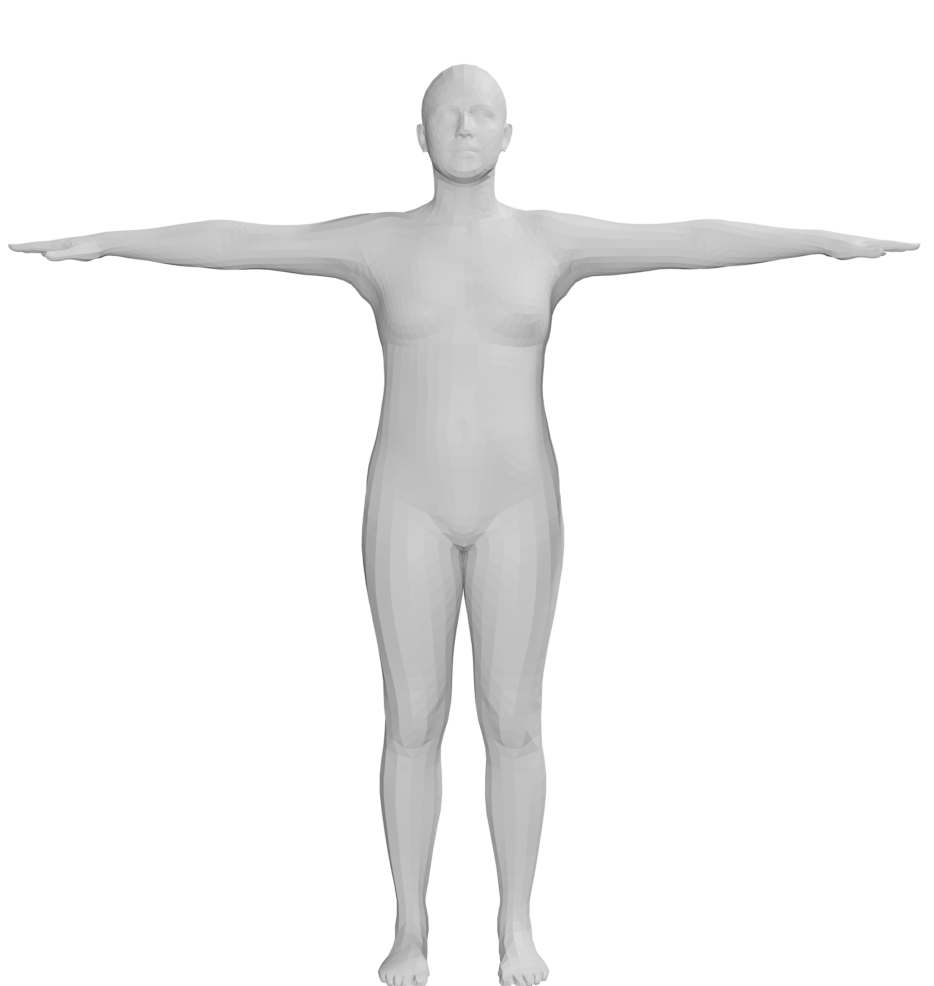
\includegraphics[width=.1\textwidth]{figures/smpl.png}};
\node[decision] (retarget) at (-1,-4) {Physics Body Model Generator};
\draw[vecArrow] (smpl) to (retarget);

\node[inner sep=0pt] (humanoid) at (2,-4){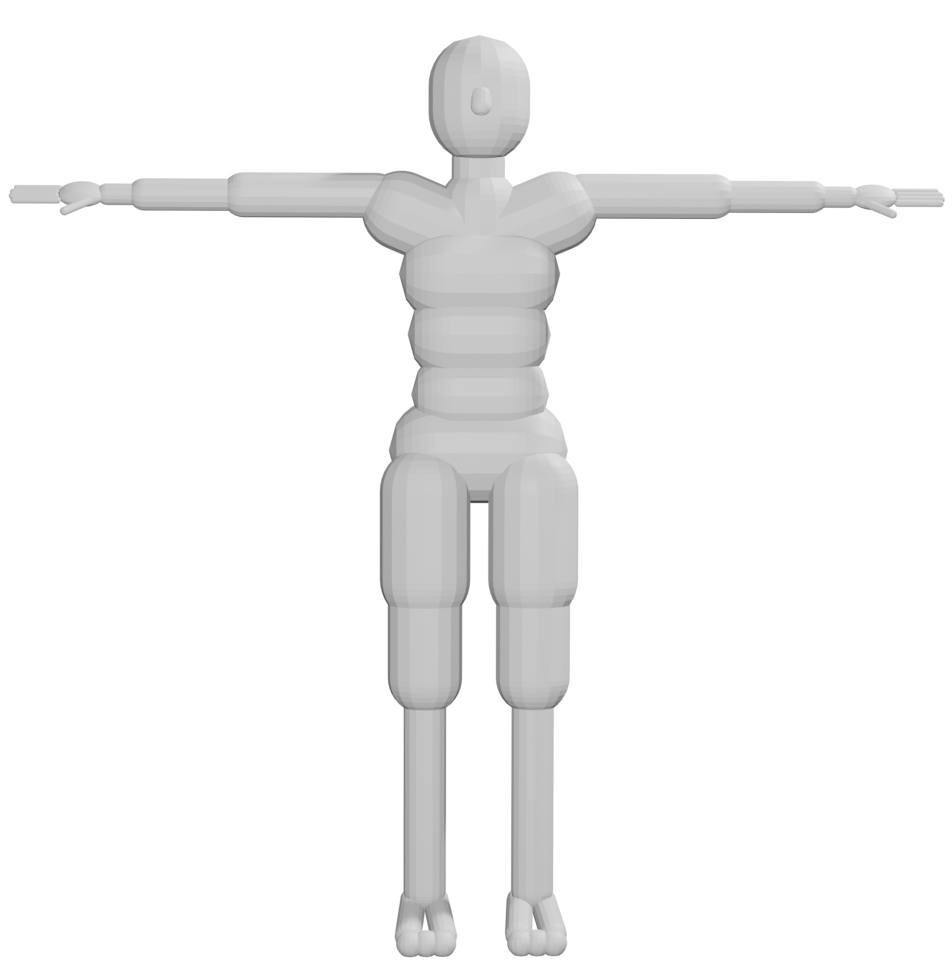
\includegraphics[width=.1\textwidth]{figures/humanoid.png}};
\draw[vecArrow] (retarget) to (humanoid);
\node[inner sep=0,minimum size=0] (k) at (5, -2.3) {};
\node[process] (lqr) at (5,-4) {iLQR Optimization};
\draw[vecArrow] (humanoid) to (lqr);
\draw[vecArrow1] (smpl2) |- (4.1,-2.3);
\draw[vecArrow] (5, -2.3) tonode[anchor=west] {$\mathbf{q}, \mathbf{v}, \mathbf{p}$} (lqr);
\node[inner sep=0,minimum size=0] (k1) at (-1, -2.3) {};
\draw[vecArrow1] (4.4, -2.3) to (-1.24, -2.3);
\draw[vecArrow] (-1, -2.28) tonode[anchor=west] {\scriptsize{$\mathbf{\beta}$}} (retarget);
\draw[innerWhite] (smpl2) |- (4.22,-2.3);
\draw[innerWhite] (k) -- (lqr);
\draw[innerWhite] (4.4, -2.3) -- (-1.18, -2.3);
% \node[process4] (lqr2) at (8,-3) {Direct Multi-person Optimization};
% \draw[vecArrow] (lqr) to (lqr2);
\node[inner sep=0pt] (final) at (9,-4){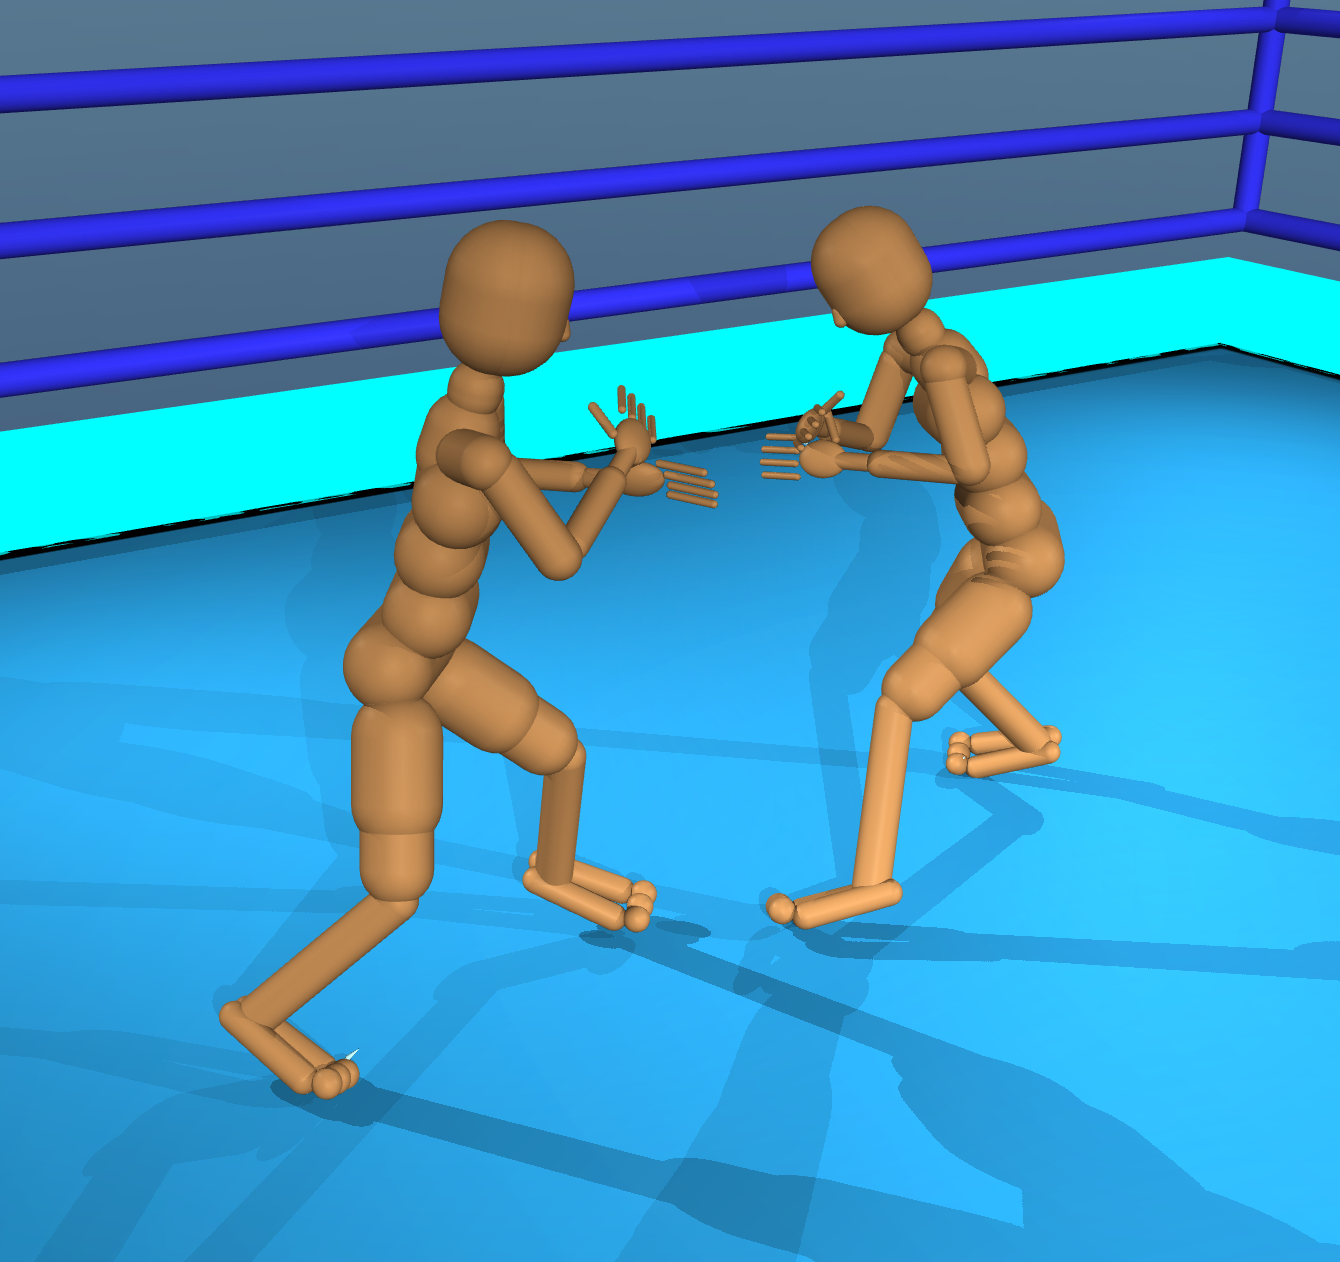
\includegraphics[width=.125\textwidth]{figures/final.png}};
\draw[vecArrow] (lqr) to (final);

\end{tikzpicture}}
\end{document}